\section{Introduction} \label{sec:background}

Successful evolutionary search depends the production of heritable, novel phenotypic variation, some of which must not be severely deleterious.
Without any heritable variation --- or even just without any viable heritable variation --- evolution stagnates.
The capacity of a population to generate viable heritable phenotypic variation is referred to as evolvability.

Different evolving systems can exhibit different degrees of evolvability.
Natural systems, in particular, are thought to generally exhibit greater evolvability than digital evolution systems \cite{mengistu2016evolvability}.
Understanding --- and replicating --- the evolvability of natural evolution is an open problem in digital evolution research \cite{mengistu2016evolvability}.
Let us examine a pair of biological examples of non-arbitrary phenotypic outcomes under mutation to build our intuition for evolvability.

A developmental constraint against certain non-viable phenotypic variation in  \textit{Drosophilia melangoster} was discovered through artificial selection experiments \cite{coyne1987lack, tuinstra1990lack}.
In these experiments,  researchers were able to successfully select for bilaterally symmetric phenotypic criteria, such as overall smaller eyes, but were unable to successfully select for bilaterally asymmetric phenotypic traits, such as different-sized eyes.
Tuinstra et al. hypothesize that the very nature of the developmental process constrains the phenotypic variation that can be observed in offspring, in this case curtailing the abundance of offspring that lack bilateral symmetry.
Specifically, they hypothesize that a lack of bilateral symmetry-breaking information during the embryological development of *Drosophila* explains the negative result of artificial selection for bilaterally asymmetric phenotypic traits.
In this way, the distribution of phenotypic diversity in offspring is biased away from (likely non-viable) asymmetric variation.

In addition to qualities that constrain against non-viable mutational outcomes, biological organisms can possess qualities that facilitate significant heritable variation for a phenotypic trait.
Somatotropin, also known as growth hormone, is well known for its widespread anabolic effects on tissues throughout the body.
Mutations affecting the regulatory pathways that regulate somatotropin production and release, the receptors and cell signaling components that mediate cellular response to somatotropin, and the protein itself all provide avenues for significant heritable variation in body size \cite{devesa2016multiple}.
Dog breeds exhibit a range of body weights spanning nearly an entire order of magnitude.
Indeed, among certain groups of dogs, much of this variation can be explained by just six genes, several of which are associated with pathways somatotropin participates in \cite{rimbault2013derived}.
The presence of hormonal signaling pathways like those somatotropin participates in can be viewed as making a broad range of heritable phenotypic variation more readily realizable via mutation.

A general consensus exists in the literature that evolvability stems from traits that facilitate the generation of \textit{novel} heritable phenotypic variation that is \textit{viable} \cite{tarapore2015evolvability}.
Tarapore et al. introduced an evolvability measure that takes a clear-eyed, simultaneous view of both of these primary aspects of evolvability \cite{tarapore2015evolvability}.
They forgo use of a scalar metric to describe evolvability, instead reporting evolvability using what they term a ``signature.''
Essentially, the signature is a two-dimensional heatmap presenting the changes in phenotypic form and fitness observed in individual offspring from a single parent.
Normalized mutual information between the phenotypic states of parent and offspring is used to quantify the amount of change in phenotypic form observed in an offspring.
Proportion decrease in fitness is used to quantify the fitness difference between parent and offspring.
For a highly evolvable individual, we would expect to see offspring occurring with significant frequency in the corner of the heatmap indicating significant change in phenotypic form with slight or no loss of fitness.
The evolvability signature provides a nuanced snapshot of evolvability, allowing for interaction between the two primary components of evolvability to be visualized.
Such information can be highly diagnostic, for example alerting researchers to phenomena that might appear falsely promising using other metrics, such as genetic changes that alter phenotypic form significantly but at great cost to fitness or genetic changes that are beneficial to fitness but fail to uncover novel phenotypic form.
Figure \ref{fig:reading_evolvability_signature} illustrates how an evolvability signature is laid out.

\begin{figure}
  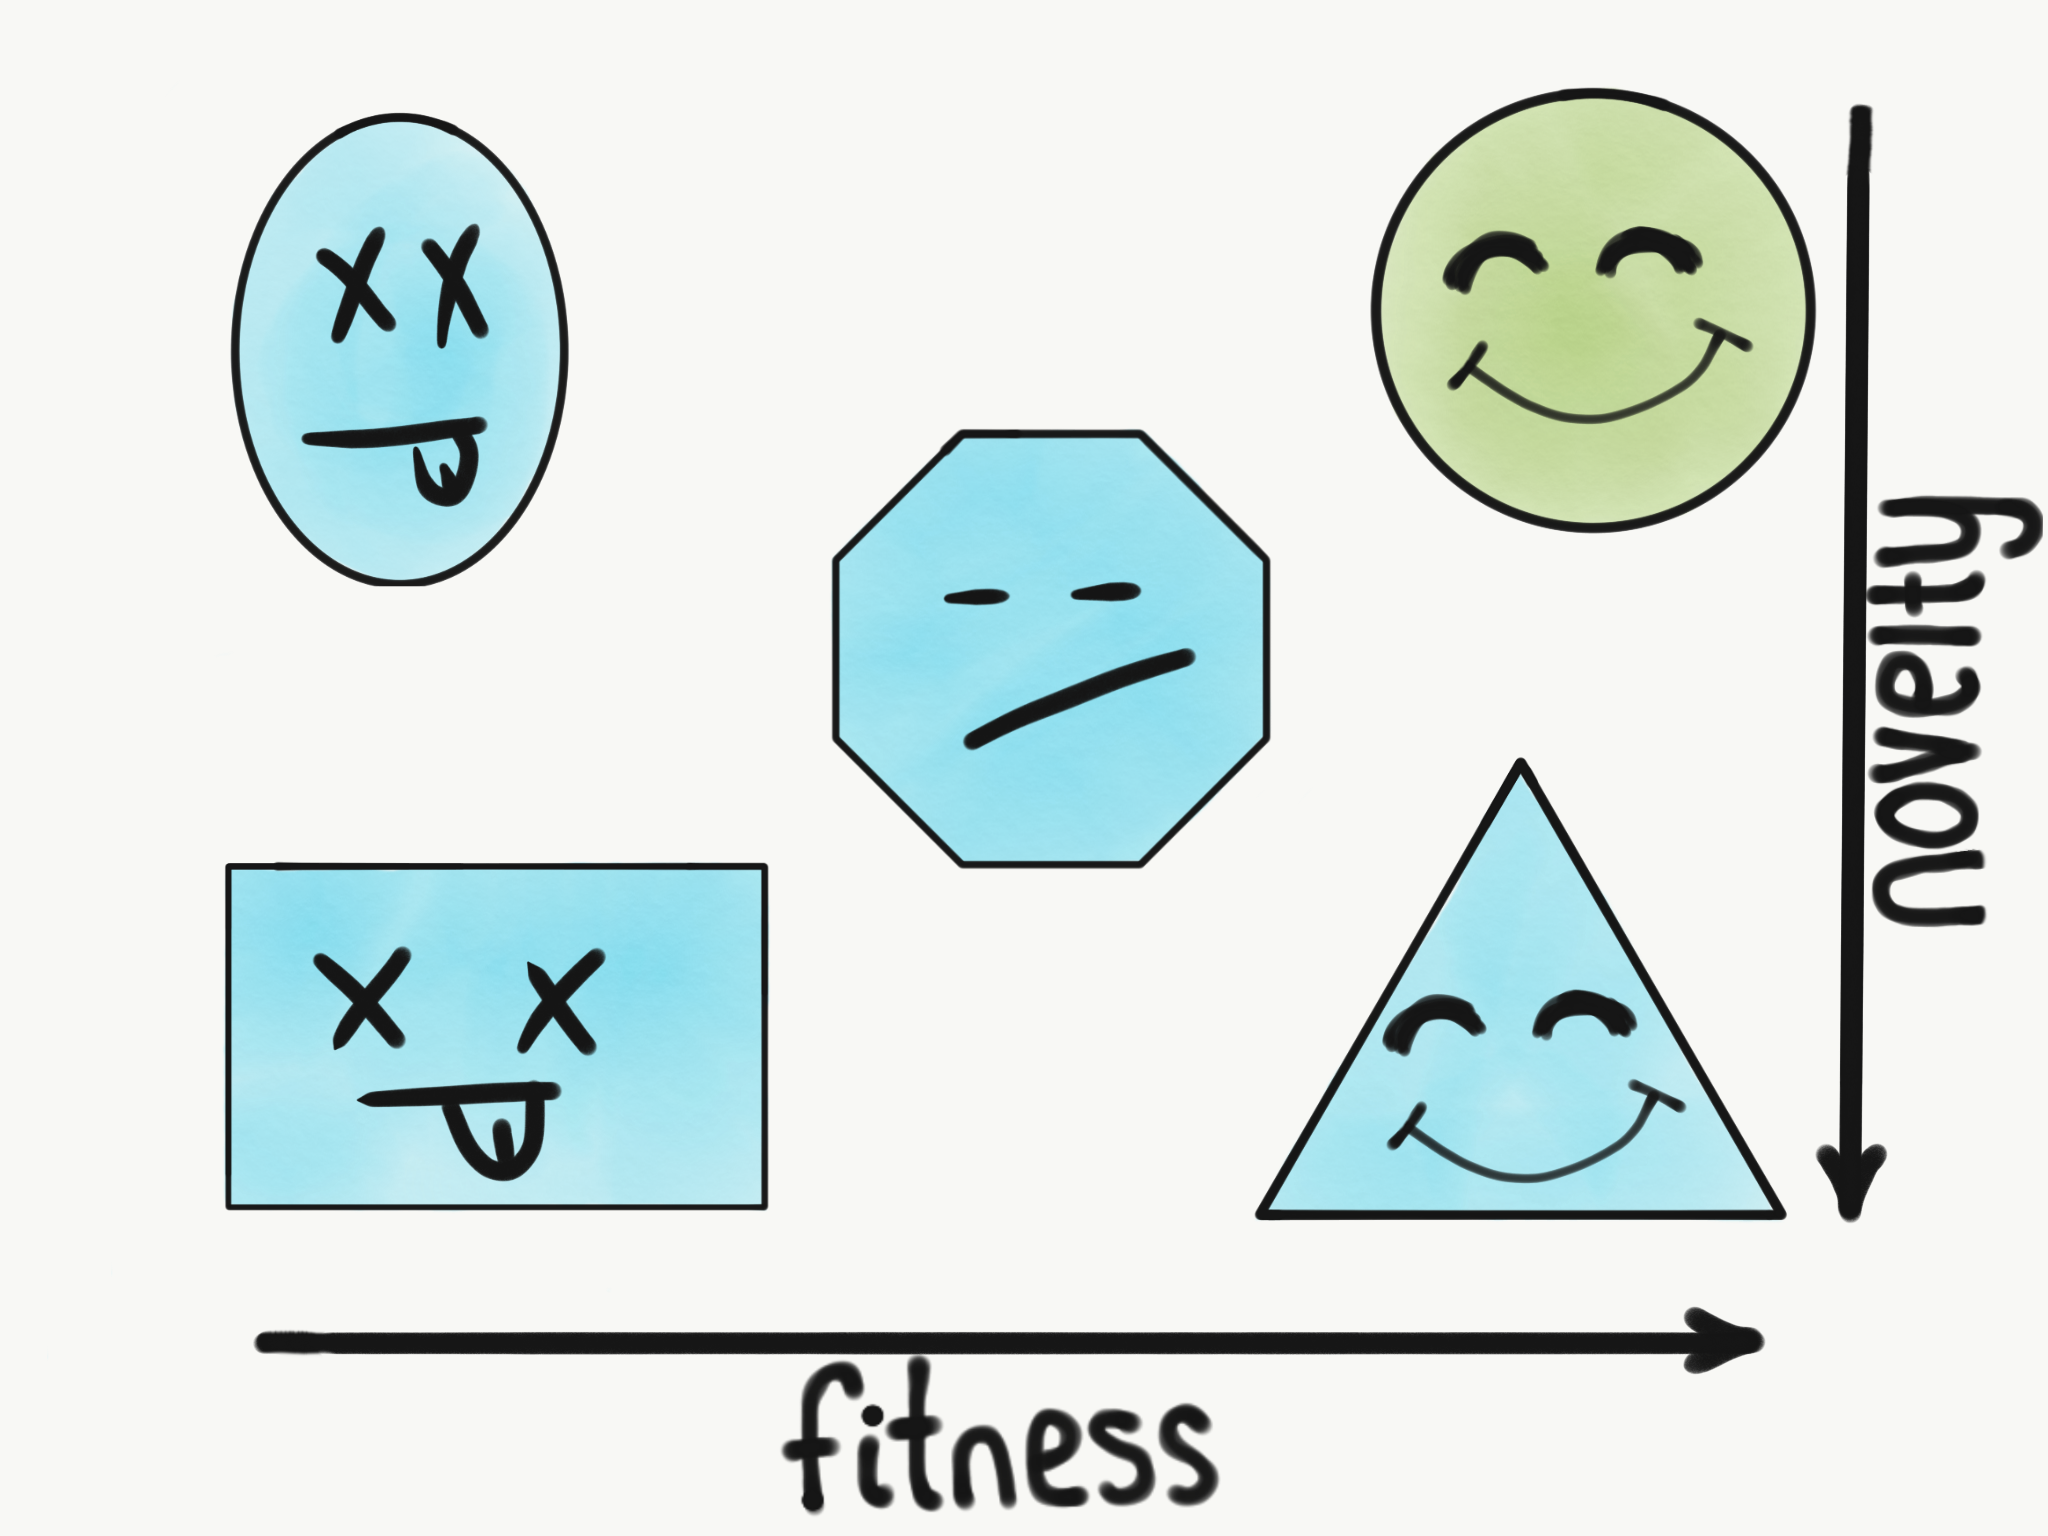
\includegraphics[width=0.8\linewidth]{img/reading_evolvability_signature}
  \caption{
    Cartoon illustration describing the layout of an evolvability signature diagram \cite{tarapore2015evolvability}.
    The parent phenotype is located in the upper right.
    Novelty increases top to bottom and fitness decreases right to left.
  }\label{fig:reading_evolvability_signature}
\end{figure}


Evolvability is desirable in artificial evolution systems for practical ends --- developing more evolvable artificial evolution systems will allow evolutionary algorithms to tackle more sophisticated problems more effectively.
Ultimately, it is hoped that artificial evolution might achieve evolvability rivaling that of natural systems \cite{mengistu2016evolvability}.
Beyond practical considerations, understanding evolvability is additionally of great scientific interest for evolutionary biologists and evolutionary computing researchers alike \cite{mengistu2016evolvability, pigliucci2008evolvability}.

\subsection{Genotype-Phenotype Map and Evolvability}

In biological science, a distinction is drawn between an organism's genotype and phenotype.
Phenotype refers to an organism's observable characteristics (morphological, behavioral, physiological, chemical, etc.) that govern its interaction with the environment and ultimately determine its fitness.
Genotype refers the heritable information that influences the phenotype displayed by the individual, i.e. the organism's DNA.
Development is the process through which an organism's genotype shapes (but does not completely determine due to environmental influence) its phenotype.
It is useful to abstract development as a mathematical function that takes genetic information as its input and outputs phenotypic characteristics.
This mathematical function representing development is referred to as the genotype-phenotype map \cite{alberch1991genes}.

The nature of the genotype-phenotype map employed in an evolving system is thought to influence that system's evolvability \cite{pigliucci2010genotype}.
It is of theoretical interest to study genotype-phenotype maps and their relation to evolvability.
In digital evolution, it is also practical interest to implement evolvable genotype-phenotype maps: more evolvable genotype-phenotype mappings enables more sophisticated digital evolution.
Let us discuss three theoretical constructs that are useful to understanding the relationship between the genotype-phenotype map and evolvability: latent evolvability, acquired evolvability, and innate evolvability.

The terms latent evolvability and acquired evolvability were introduced by Reisinger et al. in \cite{reisinger2005towards} to discuss canalization, the ability of a population to bias the types of phenotypic variability generated among its offspring in order to exploit fitness biases specific to its environment.
It is key to observe that canalization is a ``learned'' bias, developed over the course of evolution in response to selection pressure in a particular environment \cite{reisinger2005towards}.
Latent evolvability describes a genotype-phenotype map's potential to exhibit canalization while acquired evolvability describes actual canalization exhibited by an evolving population in response to a particular fitness environment.
I introduce the term innate evolvability to describe bias towards viable variation that is inherent to a genotype-phenotype map.
For example, Clune et al. identify bias towards phenotypic regularity, which in certain environments tends to be a useful trait, as an inherent quality of indirect genetic encoding \cite{clune2008generative}.

Innate, latent, and acquired evolvability each represent an opportunity for intervention by digital evolution practitioners in pursuit of an evolvable genotype-phenotype mapping.
Researchers can manually design architecture for an evolving system (often inspired by properties and mechanisms of the developmental processes in nature) that exhibits strong innate (\cite{clune2011performance}) or latent (\cite{reisinger2005towards}) evolvability.

Indeed, hand-design of genotype-phenotype maps is common practice in evolutionary computing.
Genotype-phenotype mappings have been built that exhibit latent \cite{reisinger2007acquiring} and innate \cite{stanley2009hypercube, clune2011performance} evolvability.
These manually designed genotype-phenotype mappings have proven useful for solving complex problems with evolutionary computing \cite{woolley2010evolving}.
Unfortunately, existing manually-designed genotype-phenotype mappings tend to be domain-specific --- a scheme useful for artificial neuroevolution, for example, likely isn't useful in a linear genetic programming context.
Sophisticated genotype-phenotype mappings --- particularly those extensively mimicking low-level aspects of embryological development --- are also difficult to design and implement \cite[p 223]{downing2015intelligence}.

Selection techniques like evolvability selection (\cite{mengistu2016evolvability}), modularly varying environments (\cite{kashtan2005spontaneous}), etc. can be employed to goose evolving populations towards regions of the genotype space that bestow acquired evolvability.
Although this approach has also been demonstrated successfully, it is inherently limited by the latent evolvability of the genotype-phenotype mapping that it is employed with (\cite{reisinger2005towards}).

\subsection{Evolution and Learning}

In this article, we propose a propose a fourth approach to achieve evolvability: directly learn an evolvable genotype-phenotype mapping from a training set of phenotypes harvested from local fitness peaks in an evolutionary search space using machine learning techniques for unsupervised learning.
This idea is inspired by recent work explicitly framing evolution and evolvability in the context of learning theory \cite{kouvaris2017evolution, watson2016can}.
Watson et al. and Kourvais et al. suggest that because phenotypic variation generated under mutation and recombination is fundamentally shaped by an evolutionary history, that the analogy of evolution to a learning system that exploits past experience to make informed decisions.
The key point is that undirected genetic variation can lead to structured phenotypic variation under a genotype-phenotype map that is shaped by evolutionary history \cite{watson2016can}.
Kourvais et al. specifically suggest that evolution might learn to generalize from past experience, essentially learning the structural regularities of phenotypes that were successful in the past and generating new phenotypes that are variations on that theme \cite{kouvaris2017evolution}.

\subsection{Autoencoder Neural Networks}

This techniques we propose to learn evolvable genotype-phenotype mappings rely on autoencoder neural networks.
We will take a brief detour to introduce these tools.

Autoencoders are artificial neural networks that are trained to regurgitate as output the input that they were provided.
Such networks are used to discover efficient lower-dimensional codings for datasets and, more recently, as method for generative modeling \cite{liou2014autoencoder, kingma2013auto}.
We will use two specific types of autoencoders: the bottlenecked autoencoder and the denoising autoencoder.

\begin{figure}
  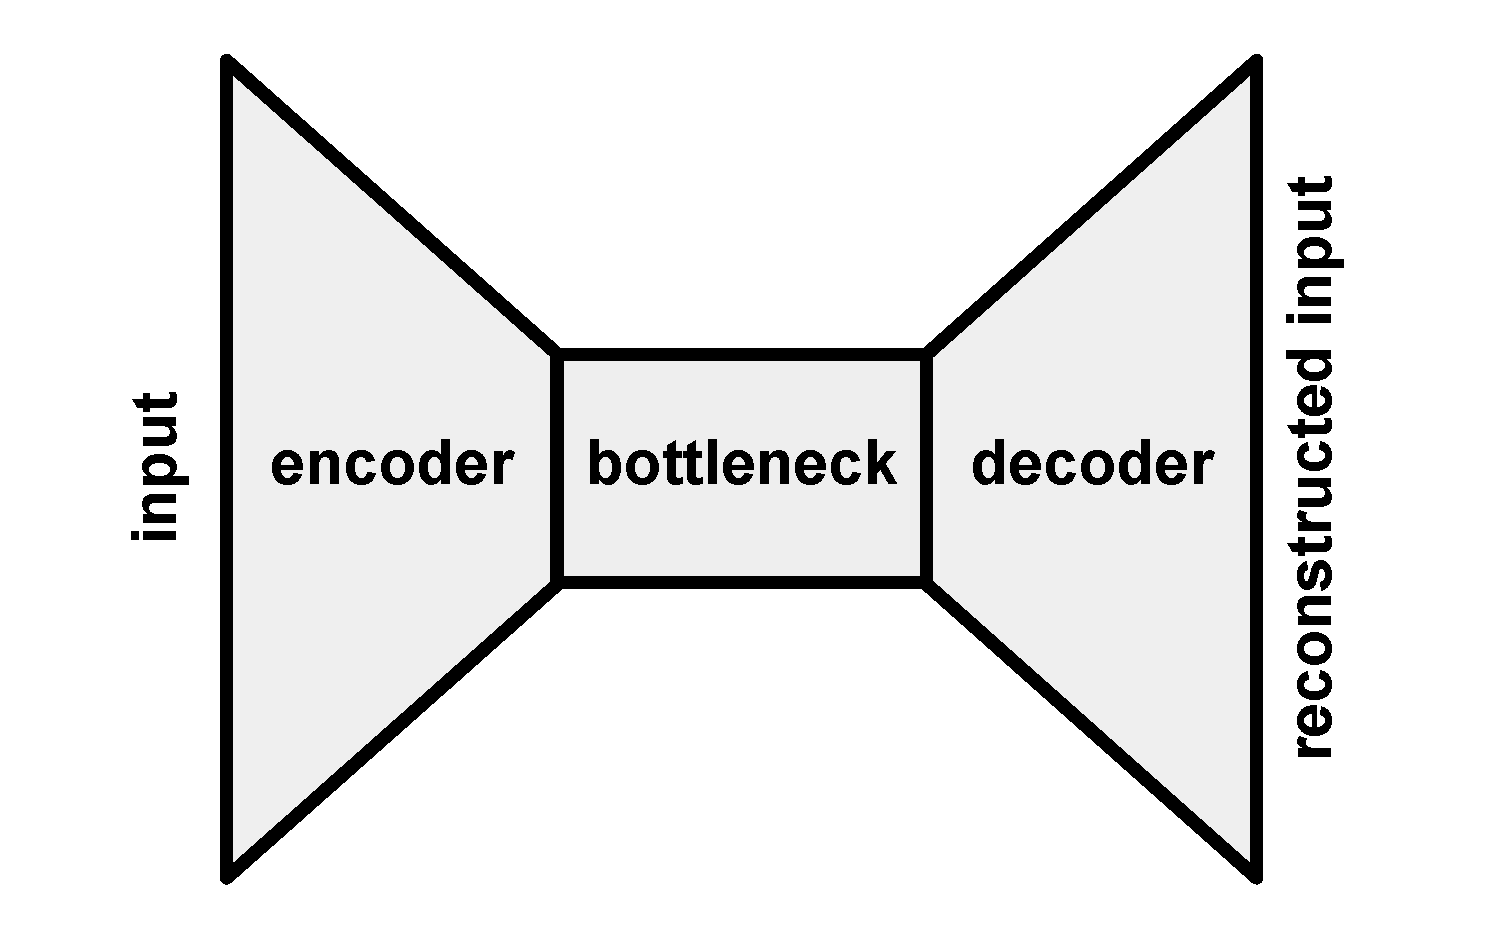
\includegraphics[width=0.5\linewidth]{img/bottleneck}
  \caption{Schematic of a bottlenecked autoencoder.}
  \label{fig:bottleneck}
\end{figure}


Figure \ref{fig:bottleneck} provides a schematic depiction of a bottleneck autoencoder.
This autoencoder has a small layer in the middle that information must pass through to reach the output.
Thus, the autoencoder is forced to learn a compact representation for the inputs it is trained with that can pass through the bottleneck.
The part of the autoencoder that precedes the bottleneck is called the encoder and the part that follows is called the decoder.

\begin{figure}
  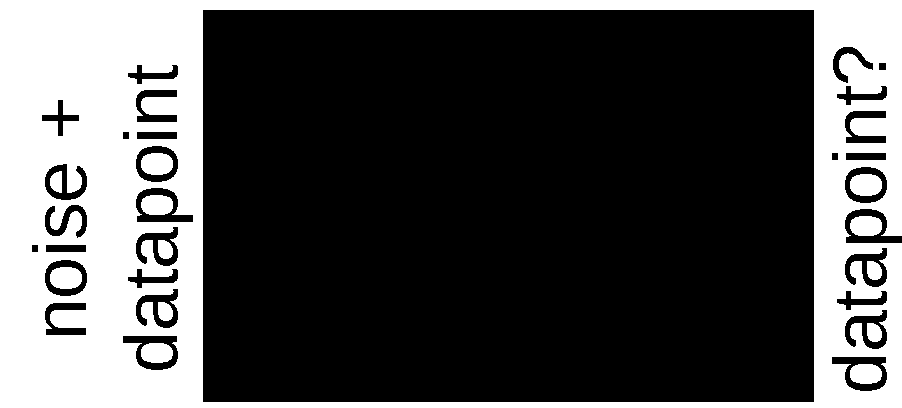
\includegraphics[width=\linewidth]{img/denoiser}
  \caption{
    Schematic of a denoising autoencoder.
  }\label{fig:denoiser}
\end{figure}


Figure \ref{fig:denoiser} provides a schematic depiction of a denoising autoencoder.
These autoencoders are trained to take noisy input and, from that noisy input, recover a signal in its original unadulterated form.

\subsection{Learning an Evolvable Genotype-Phenotype Mapping}

The pair of proposed techniques to automatically learn evolvable genotype-phenotype mappings are based on autoencoders trained to encode phenotypes taken from local fitness peaks spread throughout an evolutionary search space.
(These phenotypes are gathered by evolving a large number of replicate direct-encoded populations and retaining champion individuals from each population).

\begin{figure}
  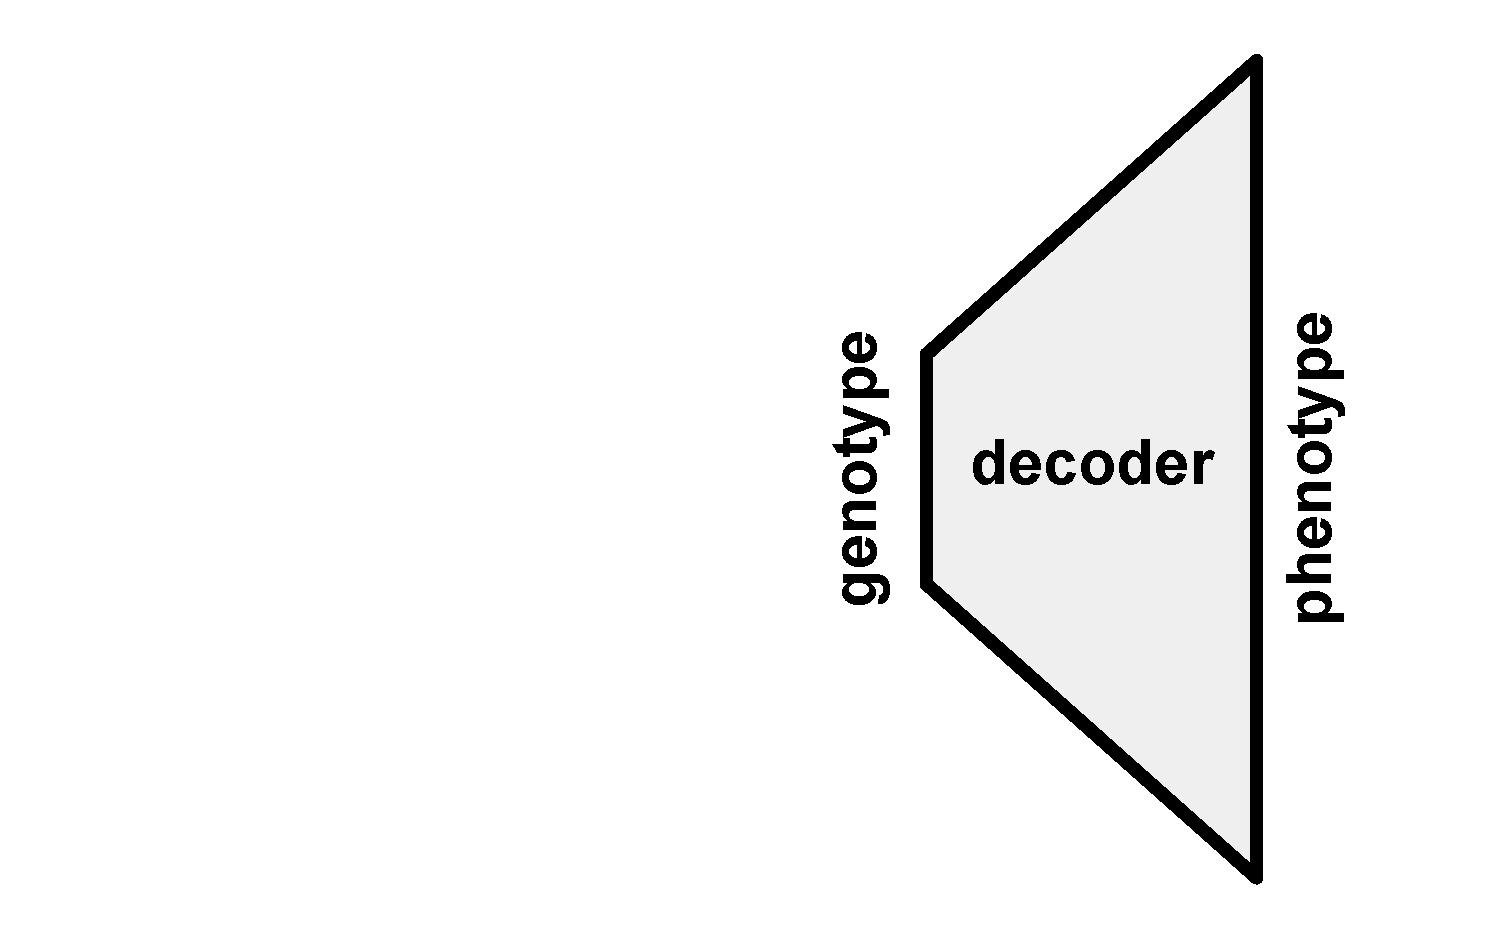
\includegraphics[width=\linewidth]{img/bottleneck_map}
  \caption{Schematic of a genotype-phenotype map constructed with a bottlenecked autoencoder.}
  \label{fig:bottleneck_map}
\end{figure}


The first approach, the bottleneck map, exploits just the decoder portion of the bottleneck autoencoder.
The decoder serves as the genotype-phenotype map so the genotype is now in the bottleneck vector space while the phenotype remains in the same vector space as before.
The idea of this approach is that, because the bottleneck provides a compact representation of those high-fitness phenotypes, using the decoder as a genotype-phenotype mapping will readily allow mutation to move the phenotype between otherwise distant fitness peaks.
This approach is illustrated in Figure \ref{fig:bottleneck_map}.

\begin{figure}
  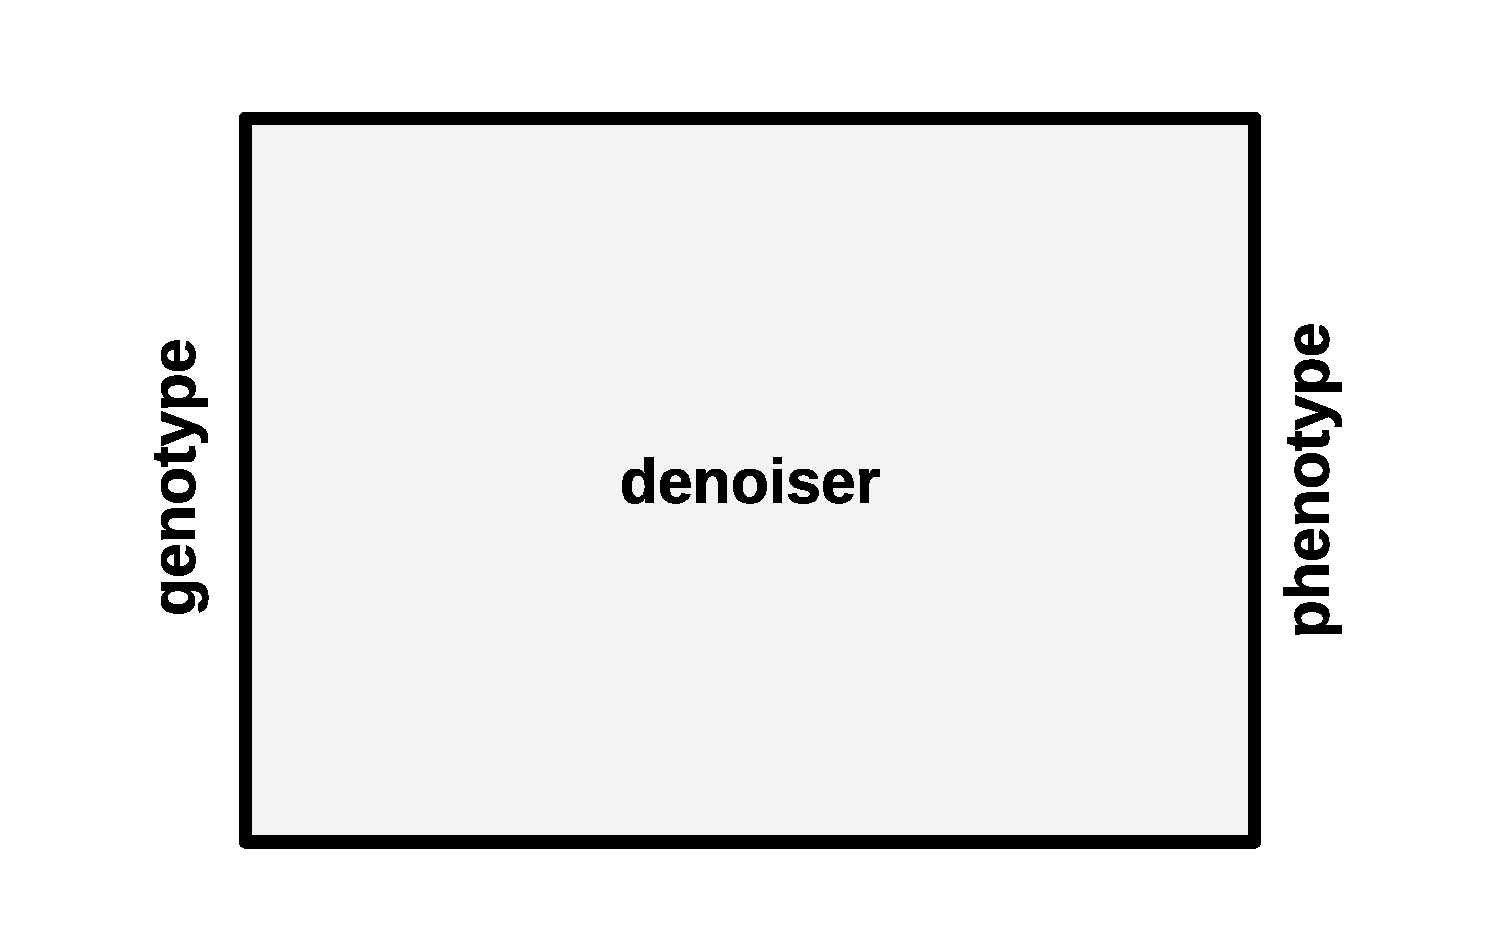
\includegraphics[width=\linewidth]{img/denoiser_map}
  \caption{
    Schematic of a genotype-phenotype map constructed with a denoising autoencoder.
  }\label{fig:denoiser_map}
\end{figure}


The second approach, the denoiser map, employs the entire denoising autoencoder would be used as the genotype-phenotype mapping.
Note that the genotype and phenotype remain in the same, equivalent vector spaces.
The idea of this design is that mutations that would otherwise be deleterious will be interpreted as noise and prevented from being expressed by the genotype-phenotype mapping.
Effectively, this mapping should flatten out the valleys between local fitness peaks to allow evolution to more readily drift between those local fitness peaks.
This approach is illustrated in Figure \ref{fig:denoiser_map}.

Ultimately, it is hoped that these techniques will prove themselves to be useful methods to achieve automatic design of highly evolvable genotype-phenotype mappings in digital evolution.
